\chapter{Sinterizzazione}\label{chp:Sinterizzazione}
Permette di realizzare oggetti a partire da polveri di un
materiale.

\begin{quote}
\emph{Perché sfruttare la sinterizzazione?}
\end{quote}

I motivi sono molteplici e possono essere:
\begin{itemize}
\item controllo accurato della struttura richiesta;
\item controllo della composizione chimica;
\item formabilità;
\item Quando non si vogliono macrosegregazioni;
\item realizzare dei componenti in materiali con temperatura di 
fusione particolarmente alta.
\end{itemize}

A differenza di altre lavorazioni è necessario parametrizzare la 
forma delle polveri, in quanto da quei parametri si possono ottenere 
le caratteristiche meccaniche del lavorato finale.
Inoltre la forma della polvere può essere determinante sulla
lavorazione.

Per i prodotti lavorati in sinterizzazione si parla di \eng{Net-
Shape}: ovvero, la lavorazione porta dei semilavorati già molto 
vicini alla forma finale di vendita del prodotto.
Ciò permette di usare tutto il materiale, senza avere sprechi dovuti
a delle lavorazioni che per ottenere la forma finale, devono 
eliminare parte di esso.

Data la lavorazione è possibile controllare la porosità del prodotto
come si vedrà successivamente.
In generale non si ottengono particolari caratteristiche meccaniche
anche se alle volte si possono ottenere delle caratteristiche 
migliori di altre lavorazioni già viste.

Bisogna prestare attenzione al discorso della porosità: troppa
porosità residua può essere punto di fragilità del materiale portando
alla formazione di cricche.
In più non sono facili da lavorare in post-produzione. Quindi il 
processo di produzione deve essere \eng{near net-shape} il più
possibile.

\section{La lavorazione}
Alla figura \ref{fig:ProcSint} sono riportati i principali
possibili processi per le lavorazioni di sinterizzazione.

\begin{figure}
\centering
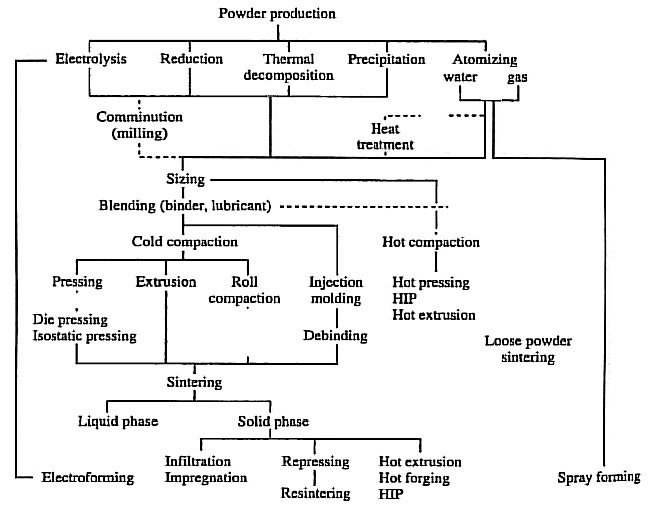
\includegraphics[width = \textwidth]{ProcSint}
\caption{Processi di produzione in sinterizzazione}
\label{fig:ProcSint}
\end{figure}

In generale il processo di sinterizzazione deve passare attraverso 
tre principali processi:

\begin{center}
\smartdiagram[sequence diagram]{Produzione Polveri, Compattazione, Sinterizzazione}
\end{center}

Sarà anche la la sequenza delle trattazioni successive.

\subsection{Produzione delle polveri}
La produzione delle polveri a partire da un semilavorato è un'operazione importate dato che, dalla caratterizzazione della polvere, si possono ottenere diverse proprietà meccaniche.
Come illustrato dalla figura \ref{fig:ProcSint}, le polveri possono essere prodotte in diverse modalità tipo:
\begin{description}
\item[Estrazione] Da un blocco di materiale si ottengono le particelle tramite:
	\begin{description}
	\item[Riduzione in ossido] dalla quale si disgrega il materiale di partenza per ossidazione e si ottiene una \textit{torta porosa}.
	\item[Decomposizione chimica] Tramite agenti chimici che attaccano il materiale di partenza si ottengono delle particelle aguzze.
	\item[Elettrolisi] Anche in questo caso si tratta di un attacco chimico e produce depositi che devono subire una successiva macinazione.
	\item[Precipitazione per soluzione acquosa] Il deposito si ha per precipitazione a partire da una soluzione liquida.
	\end{description}
\item[Deposizione] Si vaporizza il metallo per poi farlo precipitare dopo un raffreddamento. Ciò impone di prestare attenzione a quale sia la temperatura di fusione ed eventuale vaporizzazione del metallo.
\item[Atomizzazione] Può essere svolta in diverse modalità. Si sfrutta la formazione di piccole gocce di materiale fuso che, una volta raffreddate, possano diventare polvere a grana molto fine. 
In industria sono tre le modalità principalmente utilizzate, come illustrato alla figura \ref{fig:Atom}:
	\begin{enumerate}
	\item Frammentazione per fluido, in figura \ref{fig:Atom1}: dove viene fatto colare il fuso da un ugello che già forma delle gocce. Viene, poi, spruzzato del fluido, che può essere acqua o aria, per frammentare il fuso in piccole particelle. In genere si ha una relazione tipo $p_{\text{fluido}} \nearrow$ allora $D_{\text{polvere}} \searrow$.
	Bisogna comunque considerare che le particelle saranno ossidate per via del raffreddamento tramite fluido. Che può essere positivo nel caso del alluminio perché si forma allumina, non positivo per materiali ferrosi dove l'ossido forma strutture troppo dure e fragili, dannose per il prodotto post sinterizzazione.
	\item Atomizzazione centrifuga, in figura \ref{fig:Atom2}: Il colato viene spruzzato, come prima, sopra un cilindro rotante raffreddato. La forza centrifuga imposta dal cilindro alle gocce separa ulteriormente il colato formando particelle più fine. Le quali verranno raffreddate ulteriormente per il fatto che all'impatto col cilindro trovano una superficie molto più fredda.
	\item Atomizzazione con elettrodo rotante, in figura \ref{fig:Atom3}: grazie all'elettrodo si realizza un arco elettrico col materiale da polverizzare che di conseguenza si consumerà producendo la polvere. Si pone in rotazione il materiale da polverizzare. Con questo processo si ottengono delle particelle particolarmente pulite da ossidi e molto fine.
	\end{enumerate}
\item[Produzione di fibre] Non è insolito produrre delle fibre invece di polveri, le modalità sono diverse, simili a quelle viste per ottenere le polveri e sono illustrate alle figure \ref{fig:Fiber}. Le fibre hanno dei tempi di raffreddamento molto veloce: ottenendo strutture amorfe per via del fatto che il materiale non ha tempo di realizzare le strutture cristalline o non completamente.
Se si vuole ottenere fibre a partire dalla frantumazione del blocco di partenza, allora è necessario che il materiale si molto fragile.
\end{description}

Una volta ottenute le polveri e/o fibre, si passa alla caratterizzazione delle tali: ciò per mette di capire quale sia il miglior processo per la produzione.

\begin{figure}
\centering
\subfloat[][\emph{Atomizzazione per frammentazione a fluido}\label{fig:Atom1}]
{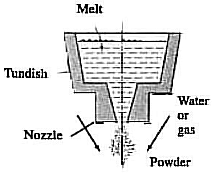
\includegraphics[width = 0.3\textwidth]{Atom1}}\:
\subfloat[][\emph{Atomizzazione tramite cilindro rotante raffreddato}%
\label{fig:Atom2}]
{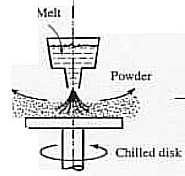
\includegraphics[width  = 0.3\textwidth]{Atom2}}\:
\subfloat[][\emph{Atomizzazione tramite elettrodo}\label{fig:Atom3}]
{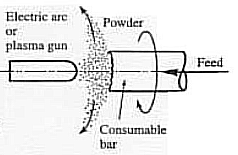
\includegraphics[width = 0.3\textwidth]{Atom3}}\\
\subfloat[][\emph{Ottenimento delle fibre per frantumazione}\label{fig:Fiber1}]
{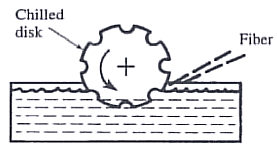
\includegraphics[width = 0.3\textwidth]{Fiber1}}\:
\subfloat[][\emph{realizzazione di fibre tramite cilindro rotante raffreddato}%
\label{fig:Fiber2}]
{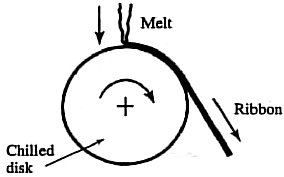
\includegraphics[width  = 0.3\textwidth]{Fiber2}}\:
\subfloat[][\emph{laminazione del fuso per ottenere delle fibre}\label{fig:Fiber3}]
{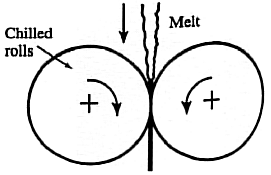
\includegraphics[width = 0.3\textwidth]{Fiber3}}
\caption{Principali modalità di atomizzazione e realizzazione delle fibre}
\label{fig:Atom}
\end{figure}

\subsubsection{Caratterizzazione delle polveri}
Una prima caratterizzazione può essere in base alla \textbf{morfologia} della polvere.
La caratterizzazione è normata tramite ISO e si suddivide in due principali dimensioni:
\begin{description}
\item[Forma] Le principali forme nella normativa sono:
	\begin{itemize}
	\item sferoidali,
	\item nodulari,
	\item irregolari,
	\item laminari,
	\item aciculare,
	\item dendritiche,
	\end{itemize}
\item[Dimensioni] si vogliono delle particelle di dimensioni né troppo grandi né troppo piccole: si vogliono abbastanza fine per evitare la formazione di macro-segregazioni; si vogliono sufficientemente grandi per evitare che diano problemi di gestione delle polveri.
Le dimensioni vengono "misurate" tramite una serie di setacci che ne danno la distribuzione.
\end{description}

\paragraph{Particelle sferoidali} vengono particolarmente apprezzate per il fatto che nel trasporto e nella gestione hanno un ottimo scorrimento. In più hanno il migliore rapporto superficie/volume che è molto importante per la formazione dei legami inter-granulare.
Presentano una minore superficie di contatto per legare con altre particelle. È anche importante per evitare di legare con impurità.
Il vantaggio di avere un ottimo scorrimento permette di ottenere, ad un primo impaccamento, la densità più alta. Dunque una minore porosità interna.
Le particelle non devono essere troppo fine perché possono dare problemi per la loro gestione: possono dare ignizione di fiamme, si possono infilare ovunque dando problemi ai macchinari, possono legarsi con impurità più facilmente.

Altri parametri con cui vengono misurate le polveri sono:
\begin{description}
\item[Area specifica della superficie] indica quanta area è a disposizione per creare legami con altre particelle e con eventuali impurità.
\item[Densità vera] sarebbe la densità del materiale da cui si sono ottenute le polveri.
Viene usata come riferimento per stimare quanta densità si ottiene post compattazione e sinterizzazione.
\item[Densità apparente] Dato uno stampo, la densità della polvere che viene messa nello stampo senza alcun sistema di compattazione.
\item[Densità disponibile] è la densità della polvere che, posta nello stampo, le viene imposta una compattazione non per realizzare il verde.
\item[Capacità di flusso] indica la portata nell'unità di tempo in un imbuto standardizzato.
Si può misurare anche misurare tramite l'angolo di cono che forma lasciando cadere le polveri in un punto.
\end{description}

In generale, tutte queste caratteristiche dipendono da: forma delle particelle, attrito tra le particelle, distribuzione delle dimensioni.

\subsection{Preparazione delle polveri}
Una volta ottenuti le polveri si susseguono i seguenti passaggi:
\begin{enumerate}
\item \textbf{Classificazione}, come visto in precedenza secondo la normativa ISO.
\item \textbf{Separazione degli agglomerati}: di solito realizzata tramite macinazione con la possibilità di modificarne la forma, con conseguente incrudimento del materiale. Arrivando ad avere una modifica delle caratteristiche meccaniche.
\item \textbf{Condizionamento} il cui obbiettivo principe è quello di gestire gli ossidi.
L'ossido è in generale un composto tenace che compromette tra particelle vicine.
In più il condizionamento permette una corretta gestione delle polveri che risulta essere particolarmente critica.
\item \textbf{Miscelazione} il discorso della miscelazione verrà affrontato più nel dettaglio al paragrafo successivo.
\end{enumerate}

\subsubsection{Miscelazione}
La miscelazione viene sfruttata per raggiungere determinati obbiettivi.
\begin{enumerate}
\item Mescolare grani di polveri di diverse dimensioni per garantire minore porosità residua;
\item Modificare la reologia delle tensioni applicate;
\item Modificare o cercare diversa densità;
\item Composizione o caratteristiche funzionali: come ad esempio la fusione di materiali non miscibili tra loro tipo: Fe-Cr.
\item Aggiunta di additivi: come lubrificanti per permettere alla polvere di scivolare meglio,
coadiuvanti della sinterizzazione. Leganti per mantenere le particelle legate tra loro in verde. Sospensioni usate per lo stampaggio ad iniezioni. Essicatura spray.
\end{enumerate}

\subsection{La compattazione}
Al termine della compattazione si ha il così detto \textbf{corpo in verde} cioè un semilavorato sufficientemente resistente per poter essere maneggiato ma non ancora in legame definitivo. 

Al grafico \ref{fig:DimPart_Density} si confronta la dimensione delle particelle fine e grossolane immesse nello stampo per ottenere una certa densità apparente.
Mentre, al grafico \ref{fig:Compattazione} viene riportata la resistenza meccanica in funzione della pressione di compattazione.

\begin{figure}
\centering
\subfloat[][\emph{Densità relativa alla dimensione delle particelle immesse nello stampo}\label{fig:DimPart_Density}]
{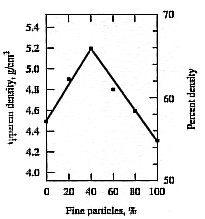
\includegraphics[width = 0.4\textwidth]{DimPart_Density}}\quad
\subfloat[][\emph{Resistenza del verde in funzione della pressione di compattazione}\label{fig:Compattazione}]
{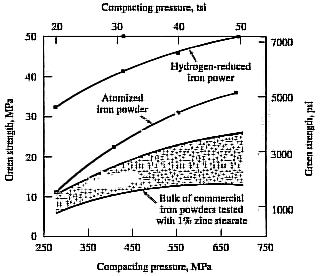
\includegraphics[width = 0.4\textwidth]{Compattazione}}\\
\subfloat[][\emph{Pressatura a freddo semplice della polvere}\label{fig:PressaFreddo}]
{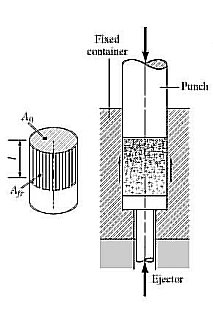
\includegraphics[width = 0.3\textwidth]{PressaFreddo}}\quad
\subfloat[][\emph{Tecniche di diminuzione del gradiente di pressione sul compattato}\label{fig:PressaFreddoMigliore}]
{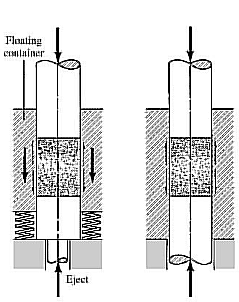
\includegraphics[width = 0.6\textwidth]{PressaFreddoMigliore}}
\caption{Parametri da considerare durante la compattazione della polvere e compattazione a freddo}
\label{fig:ParamCompattazione}
\end{figure}

\subsubsection{Come compattare?}
\paragraph{Pressatura a freddo}
La pressione sarà massima vicino al punzone e man mano cala allontanandosi dal punzone, si evidenzia in figura \ref{fig:PressaFreddo} dalle particelle più raffittite in vicinanza del punzone e via via più "rarefatte".
Per migliorare la compattazione si aumentano i numeri di punzoni: nel senso che si fa in modo di avere un doppio punzone oppure di avere una matrice flottante, sono i casi delle figure \ref{fig:PressaFreddoMigliore}.

La resistenza in verde serve per poter spostare il materiale nella linea di produzione.
La densità del pezzo arriva fino a $90\%$ della densità vera. Ciò è vero solo se l'altezza è piuttosto sottile. Altrimenti sono necessarie altre tecniche di compattazione.

A titolo esemplificativo, alla figura \ref{fig:PressaturaComplicata} Viene riportata una pressatura per un oggetto con diversi particolari.
A dimostrazione che la compattazione può essere eseguita per forme molto articolate.

\paragraph{Pressatura idrostatica}
si impongono delle compressioni idrostatiche da più direzioni per migliorare la compattazione.
In generale si utilizza uno stampo elastico, che successivamente viene messo in pressione con un fluido.

La varietà di forme ottenibili con queste tecniche è più alta per via del fatto che si riesce a compattare meglio la polvere in più direzioni.
Aumenta considerevolmente il tempo ciclo $t_c$ perché gli stami devo no essere preparati e portati in pressione. Le figure \ref{fig:PressaIdrostatica} è un esempio.
Tempi ridotti si hanno nel caso della pressatura a sacco asciutto (seconda delle figure \ref{fig:PressaIdrostatica}) ma diminuisce il numero di forme ottenibile.
Può essere che lo stampo, in genere poliuretanico, venga scaldato per imporre più resistenza al materiale verde.

Si può pensare di aumentare la varietà di forme ottenibili con la pressatura attraverso successive lavorazioni per asportazione di polvere all'oggetto in verde.

\begin{figure}
\centering
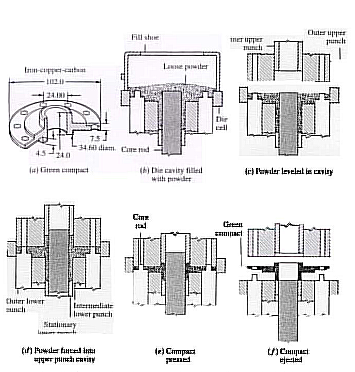
\includegraphics[width = 0.5\textwidth]{PressaturaComplicata}
\caption{Esempio di pressatura a freddo di un oggetto particolarmente complicato}
\label{fig:PressaturaComplicata}
\end{figure}

\begin{figure}
\centering
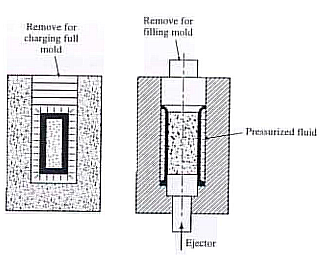
\includegraphics[width = 0.5\textwidth]{PressaIdrostatica}
\caption{Pressatura idrostatica a sacco bagnato e asciutta}
\label{fig:PressaIdrostatica}
\end{figure}

\subsubsection{Stampaggio ad iniezione}
Viene particolarmente usata per i materiali plastici, anche per la compattazione per la sinterizzazione.
Nel secondo caso è necessario che vengano aggiunti degli additivi per fluidificare le polveri permettendo un certo flusso all'interno degli stampi.
In genere vengono usati come additivi: cere e materiali termoplastici.
Ciò implica che anche le polveri abbiano dimensioni contenute.
Purtroppo, si avranno delle tolleranze geometriche e di porosità parecchio scarse post sinterizzazione.

\begin{figure}
\centering
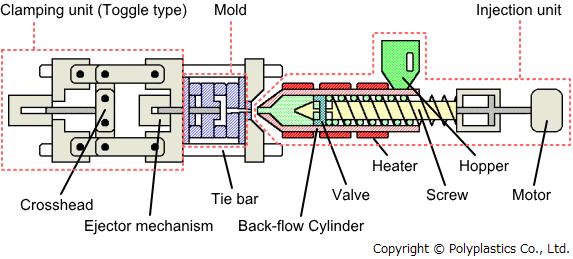
\includegraphics[width = \textwidth]{InjectionMolding}
\caption{Esempio di \eng{Injection Molding}}
\label{fig:InjectionMolding}
\end{figure}

Il processo illustrato alla figura \ref{fig:InjectionMolding} funziona in più fasi:
\begin{enumerate}
\item Una tramoggia alimenta un tubo contenente una vite infinita che ruota e trasla con moto alternativo.
\item Le particelle si scaldano a causa della viscosità e frizione reciproca.
Vale che, soprattutto per i polimerici, fluidificandosi aumenti la viscosità.
\item Man mano che più materiale viene accumulato sull'estremità della vite, questa arretra.
\item Accumulato sufficiente materiale la vite spingerà il materiale all'interno dello stampo.
\end{enumerate}

A seconda se la materia è termoplastica o termoindurente, lo stampo verrà raffreddato o riscaldato rispettivamente.

Può essere che i macchinari vengano assistiti da resistenze per aumentare la temperatura interna in fase di avvio, quando il materiale è completamente freddo o se necessario avere temperature più alte di quelle raggiungibili per effetto della sola viscosità.
Eventualmente, può essere necessario un sistema di raffreddamento per tenere controllata la temperatura.

Le forme ottenibili con questo stampaggio possono essere più complicate di quelle realizzati tramite compattazione.

\paragraph{Stampaggio di precisione}
Sono tecniche utilizzate in particolare per materiali termoindurenti.
In questo caso si ha la polvere rivestita di materiale termoindurente legato con legante solubile in acqua. Durante la sinterizzazione il materiale termoindurente sarà volatilizzato.

\subsection{Sinterizzazione}
\begin{wrapfloat}{figure}{O}{0pt}
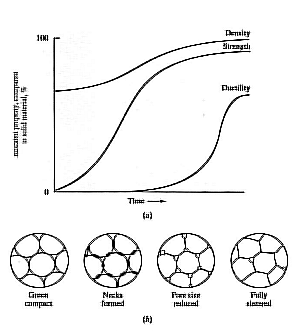
\includegraphics[width = 0.4\textwidth]{Sinterizzazione}
\caption{Caratteristiche meccaniche raggiunte dal prodotto in verde durante la sinterizzazione dopo diverso tempo e sequenza del processo}
\label{fig:Sinterizzazione}
\end{wrapfloat}
Il materiale compattato viene portato in forno e succede:
\begin{description}
\item[Asciugatura] tutti i liquidi vengono espulsi. Il tempo di asciugatura dipende dallo spessore massimo del pezzo. Non può essere troppo veloce altrimenti durante la volatilizzazione può spaccare il pezzo. Se il legante organico può essere volatilizzato come ossigeno.
\item[Sinterizzazione] L'energia ai bordi favorisce le giunzioni e la diffusione. Le temperature sono tipiche delle lavorazioni a caldo ovvero $T \approx 0.7 \div 0.9 T_m$.
Le giunzioni si allargano, diminuisce il rapporto superficie-volume si abbassa l'energia potenziale del materiale. C'è un certo ritorno per la diminuzione della porosità. Se la riduzione di volume è prevedibile, è possibile prevedere la riduzione, dunque si può stimare quanto materiale in più porre nell'oggetto in verde. La porosità compromette la resistenza a fatica.
\end{description}

Come si vede dalla figura \ref{fig:Sinterizzazione}, una volta ottenuta la fusione delle particelle, tenere il materiale per troppo tempo ad alta temperatura si rischia di aumentare troppo la dimensione dei grani, peggiorando di molto le caratteristiche meccaniche.
Si può migliorare la situazione nel caso uno degli elementi miscelati sia bassofondente.
Allora la fusione aumenta la pressione sui grani altofondenti garantendone le dimensioni piccole.
Normalmente sarebbe un difetto. In questo caso, essendo transitorio, per mette al bassofondente di mettere in pressione i grani altofondenti. Dopo avviene una reazione chimica per cui il bassofondente si lega all'altro materiale.

\begin{definition}{Capillarità}
È la capacità dei fluidi di distribuirsi in mezzo a spazi stretti a discapito della gravità. È critica la dimensione allo spazio piccolo.
\end{definition}

Spesso si conducono delle prove per stimare il ritiro in questo modo:
Ad esempio in considerazione della massa:
\begin{equation}
cost. = \rho_{green} V_{green} = \rho_{sint} V_{sint} 
\end{equation}
Allora il ritiro volumetrico può essere stimato come:
\begin{equation}
\frac{V_{sint}}{V_{green}} = \frac{\rho_{green}}{\rho_{sint}}
\end{equation}
da cui:
\begin{equation}
\text{Ritiro lineare} = \left(\frac{\rho_{green}}{\rho_{sint}}\right)^{\frac{1}{3}}
\end{equation}

I forni per la sinterizzazione possono essere:
\begin{description}
\item[Classici] Sono dei forni molto simili a quelli casalinghi, in cui tramite uno sportello frontale è possibile accedere alla camera. Sono in genere in grado di realizzare il ciclo di sinterizzazione: asciugatura, sinterizzazione, raffreddamento.
\item[Continui] tramite un nastro trasportatore i pezzi in verde attraversano diverse zone del forno corrispondenti alle fasi.
\end{description}

La porosità residua si attesta attorno a $4\% \div 15\%$.
Se interconnessa viene sfruttata per realizzare filtri e cuscinetti..
Possono rimanere zone più o meno compatte: sfruttandole per garantire determinate caratteristiche in zone maggiormente sollecitate.
Sono più difficili da lavorare per via dei continui urti tra superfici sinterizzati e utensile.

\subsection{Finiture e trattamenti termici}
\paragraph{Coniatura} è una lavorazione di forgiatura a freddo in assenz adi lubrificazione migliorando le tolleranze dimensionali.

Mentre trattamenti termici possono essere:
\subsubsection{Ricompattazione e risinterizzazione} Viene eseguito il processo più volte. Si compatta con la stessa pressione.

\subsubsection{La porosità fa comodo:}
La porosità può essere utile per diversi obbiettivi:
\begin{description}
\item[Impregnazione con olio] la porosità vengono riempite con lubrificanti per garantire lubrificazione in esercizio.
\item[Infiltrazione] non è altro che l'impregnazione con un metallo bassofondente.
\end{description}

\subsection{Compattazione a caldo}
Le polveri metalliche si conformano in modo che la porosità può essere ridotte a zero.


\moretodo[inline]{Continuare con: \textbf{Compattazione a caldo}, \textbf{Prodotti sinterizzati}, \textbf{Elettroformatura}}
